\documentclass{article}

% Language setting
% Replace `english' with e.g. `spanish' to change the document language
\usepackage[english]{babel}
\usepackage{adjustbox}
\usepackage{booktabs}
\usepackage{makecell}

% Set page size and margins
% Replace `letterpaper' with`a4paper' for UK/EU standard size
\usepackage[letterpaper,top=2cm,bottom=2cm,left=3cm,right=3cm,marginparwidth=1.75cm]{geometry}

% Useful packages
\usepackage{amsmath}
\usepackage{graphicx}
\usepackage[colorlinks=true, allcolors=blue]{hyperref}

\DeclareMathOperator*{\argmin}{arg\,min}
\DeclareMathOperator*{\argmax}{arg\,max}

\title{Exploring Hyperparameter Spaces: A Comprehensive Study of Ridge Regularization in Mean-Variance Optimization}
\author{Fernando Urbano}

\begin{document}
\maketitle

\subsection*{Material}
The code to reproduce the results can be found in: \href{https://github.com/Fernando-Urbano/efficient-frontier-regularization}{https://github.com/Fernando-Urbano/efficient-frontier-regularization}


\section{Introduction}

Markovitz's construction of the Efficient Frontier in 1952 is among the most significant improvements in quantitative finance and set the start of the Modern Portfolio Theory \cite{markowitz1952portfolio}.

The idea behind the Efficient Frontier provided an algorithm to choose optimal weights for the assets in the portfolios of hedge funds, banks, and other financial institutions.

It is part of the mean-variance optimization framework and served as the foundation for the CAPM theory of Willian Sharpe.

The original algorithm was highly praised for its simplicity accompanied, nonetheless, by a powerful conclusion: portfolio optimization depends on expected returns and risk (measured by variance) and investors aim to maximize expected returns given their levels of risk aversion. With mean-variance optimization, investors can transform their views into investment bets.

With time, the original mean-variance optimization started facing criticism due to estimation error and extremely aggressive allocation as a consequence of mathematical instability \cite{schmid2018efficient}. Nowadays, improvements in the field of Machine Learning found paths to mitigate the problem through the use of Regularization (L1 and L2) \cite{britten2013robustifying} and Resampling (Monte Carlo and Bootstrapping) \cite{bruder2013regularization}.

While the original algorithm provides a concise set of hyperparameters, modern applications with regularization techniques require extensive hyperparameter tuning and a gigantic number of possible combinations on how to address the problem. Practitioners often choose one possible set among the vast poll, given limited time to train and analyze results.

The goal of our paper is to dive deeper into the tuning of hyperparameters for RIDGE regularization, tirelessly testing possible combinations of different parameters to arrive at general guidelines on how to approach the problem and which sets generate more favorable results. We aim to provide a comprehensive study of the hyperparameter space of the RMVP, exploring the impact of the number of assets, training size, days until rebalancing (viewed as testing size), number of time-series cross-validation, and cross-validation size.

\section{Research Methodology}
\subsection{Mean-Variance Optimization}
The optimization process is based on finding the weights for assets in a given portfolio that maximize the expected return of the portfolio given a level of risk or minimize the risk of a portfolio given a level of expected return:

$$
\max_{w} \quad \mu^{T} w \quad \quad
\text{s.t.} \quad w^{T} \Sigma w \leq \sigma^{2}, \quad
\sum_{i=1}^{n} w_{i} = 1
$$

In the equation, $w$ is the vector of weights, $\mu$ is the vector of expected returns, $\Sigma$ is the covariance matrix of the returns, and $\sigma^{2}$ is the tolerated level of risk. The first constraint ensures that the risk of the portfolio is below a certain threshold, and the second constraint ensures that the investor uses 100\% (not more or less) of their capital in the allocation.

The Efficient Frontier gives the best allocation for every given risk (variance) level. The curved shape is a consequence of diversification: less than perfect correlation between assets allows for a reduction in the overall risk of the portfolio.

The Efficient Frontier has two points worth of special attention: the Global Minimum Variance Portfolio (GMV), the leftmost point, and the Tangency Portfolio.

\subsection{Global Minimum Variance Portfolio}
The Global Minimum Variance Portfolio (GMV) is the portfolio with the lowest possible variance.

Given the convex nature of the optimization problem, it is possible to find the $w_{\text{GMV}}$ with a closed form solution:

$$
{w}_{\text{GMV}} = \argmin_{w} \quad w^{T} \Sigma w \quad \quad
\text{s.t.} \sum_{i=1}^{n} w_{i} = 1
$$

$$
{w}_{\text{GMV}} = \frac{\Sigma^{-1} \mathbf{1}}{\mathbf{1}^{T} \Sigma^{-1} \mathbf{1}}
$$

In the equation, $\mathbf{1}$ is a vector of ones and $\Sigma^{-1}$ is the inverse of the covariance matrix of returns.

\subsection{Tangency Portfolio}
The Tangency Portfolio is the portfolio that maximizes the Sharpe Ratio \cite{sharpe1964capital}, a measure of risk-adjusted return, defined as the ratio of the excess return of the portfolio over the risk-free rate to the standard deviation of the portfolio (square root of the variance):

$$
\text{Sharpe Ratio (SR)} = \frac{\tilde{\mu}^{T} w}{\sqrt{w^{T} \Sigma w}}
$$

Where $\tilde{\mu} = \mu - r_f \mathbf{1}$ is the vector of excess returns, with $r_f$ being the risk-free rate.

Again, given the convex nature of the optimization problem, it is possible to find the $w_{\text{TAN}}$ with a closed form solution:

$$
w_{\text{TAN}} = \argmax_{w} \quad \frac{\mu^{T} w - r_f}{\sqrt{w^{T} \Sigma w}} \quad \quad
\text{s.t.} \sum_{i=1}^{n} w_{i} = 1
$$

$$
w_{\text{TAN}} = \frac{\Sigma^{-1} \tilde{\mu}}{\mathbf{1}^{T} \Sigma^{-1} \tilde{\mu}}
$$

\subsection{Instability and Unpredictability}
The two formulas give us the optimal weights for the given levels of risk. Any other point in the efficient frontier can be obtained by a linear combination of the GMV and the Tangency Portfolio (Figure \ref{fig:efficient_frontier}).

$$
w_{\text{optimal}} = \alpha w_{\text{GMV}} + (1 - \alpha) w_{\text{TAN}} \quad \quad \alpha > 0
$$

\begin{figure}[h]
    \centering
    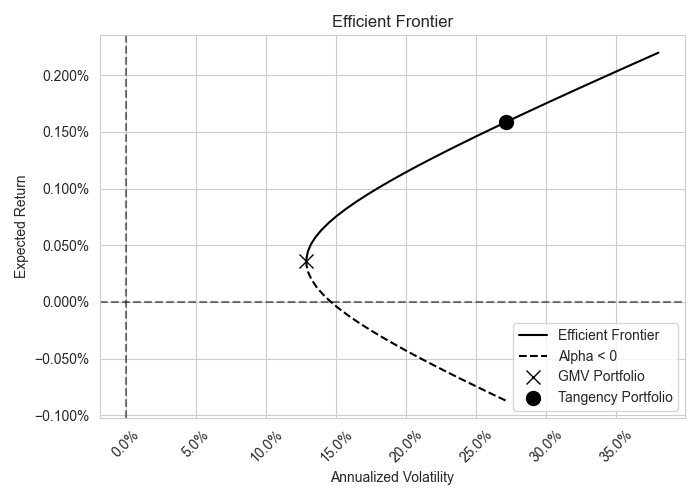
\includegraphics[width=0.8\textwidth]{graphics/illustrations/efficient_frontier.png}
    \caption{Efficient Frontier as a linear combination of the GMV and the Tangency Portfolio}
    \label{fig:efficient_frontier}
\end{figure}

However, the process of estimating expected returns and the covariance matrix from historical data encounters significant challenges. These estimates are inherently prone to inaccuracies. Specifically, returns exhibit minimal or no autocorrelation, resulting in a high level of unpredictability. While the covariance matrix's estimates are marginally more reliable, the high dimensionality of portfolio optimization exacerbates the impact of even minor estimation errors, leading to substantial discrepancies in the optimization outcomes and final portfolio allocation.

More specifically, the errors are magnified by the $\Sigma^{-1}$ term in the formulas. The inverse of the covariance matrix is highly sensitive to small changes in the estimates, given its high condition number (ratio of the largest to the smallest eigenvalue of the matrix), which serves as a measure of how much the output of the matrix changes due to small changes in the input. This results in extreme optimal weights, with large allocations in few assets (long and short).

In simpler words, a small difference between the historical and future excess returns ($\tilde{\mu}$) or the covariance matrix ($\Sigma$) leads to a large difference in the optimal weights between the training period and the future period.

\subsection{Ridge Regularization}
Ridge Regularization is a technique used to mitigate the problem of instability in the optimization process, by adding a penalty term. The optimized point of minimum variance with RIDGE is called the Regularized Minimum Variance Portfolio (RMVP).

$$
w_{\text{RMVP}} = \argmin_{w} \quad w^{T} \Sigma w + \lambda \|w\|^{2} \quad \quad
\text{s.t.} \sum_{i=1}^{n} w_{i} = 1
$$

The $\lambda$ term is the hyperparameter that controls the trade-off between the variance of the portfolio and the penalty term. As in regression problems, Ridge has the advantage of providing a closed-form solution:

\begin{align*}
w_{\text{RMVP}} = \argmin_{w} & \quad w^{T} \Sigma w + \lambda w^T w \quad \quad \\
                & \quad w^{T} \Sigma w + w^T \lambda I w \quad \quad \\
                & \quad w^{T} (\Sigma + \lambda I) w \quad \quad \\
\end{align*}

The problem is now again a quadratic form, and the solution is:

$$
w_{\text{RMVP}} = \frac{(\Sigma + \lambda I)^{-1} \mathbf{1}}{\mathbf{1}^{T} (\Sigma + \lambda I)^{-1} \mathbf{1}}
$$

The algorithm reduces the extreme allocations in few assets and decreases the sensitivity of the optimization process to small changes in the estimates.

In practice, the solution vector $w_{\text{RMVP}}$ penalty value is defined by how much the individual weights differ from the equal weight allocation of of $1/n$, where $n$ is the number of assets in the portfolio. Namely, The penalty term in RIDGE is a function of the Euclidean Norm of the vector of weights, which is minimized when $w_i = 1/n$ for all $i$ (Figure \ref{fig:euclidean_norm}).

\begin{figure}[h]
    \centering
    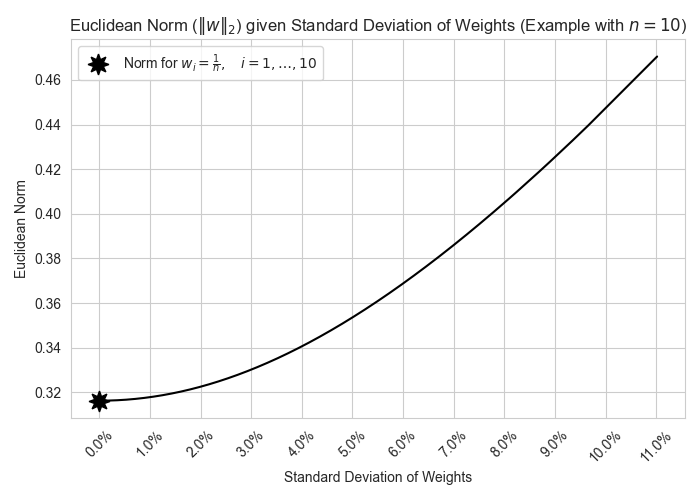
\includegraphics[width=0.8\textwidth]{graphics/illustrations/euclidean_norm.png}
    \caption{Euclidean Norm as a Function of Weights' Standard Deviation}
    \label{fig:euclidean_norm}
\end{figure}

\subsection{Methodology}
In this paper, we explore the hyperparameter space of the RMVP. Using the point of Minimum Variance steady of the Tangency Portfolio is viewed as a better approach, given that historical returns are not good predictors of future returns and we intend to remain agnostic about more other predictions models results, given that the focus should remain in the exploration of the hyperparameter of the mean-variance optimization \cite{campbell2008predicting}.

In our tests, we use the conventional format of the regularized optimization problem. Given the selected assets and training data, we use time-series cross-validation to find the optimal $\lambda$ for the RMVP selecting based on the Sharpe Ratio performance. After have chosen the optimal $\lambda$, we calculate $w_{\text{RMVP}}$ in the training sample and see their performance in the testing sample.

The hyperparameter space tested is defined by the following parameters:
\begin{itemize}
    \item Choice of number of assets $n$: 5, 10, 12, 17, 30.
    \item Choice of training size $T$ in days: 63, 126, 252, 504.
    \item Choice of testing size $t$ in days (how long the portfolio will run until a new optimization is calculated): 5, 10, 21, 42, 126, 252.
    \item Choice of number of time-series cross-validation $n_{cv}$: 1 to 8.
    \item Choice of cross-validation size $t_{cv}$ as a percentage of the training size: 50\%, 75\%, 100\%, 125\%, 150\%.
\end{itemize}

The $\lambda$'s tested are always in the range of $[0, 3]$ with a step of $0.10$ (where $\lambda = 0$ is the GMV). Before running the simulations, we tested the range in which the optimal $\lambda$'s are found, and limit the search until $3$ given that the optimal is always below this threshold. Convex optimization approaches were also tested for $\lambda$ with gradient descent, but led to unsatisfactory results, given the non-convex nature of the loss function with respect to $\lambda$.

Each of 5,600 combinations in the simulation runs from January 1st 2000 to December 31st 2022, totalizing 4.5 million calculations. As a result, we have 5,600 testing portfolios, each with 23 years of data.

The simulations provide answer to questions such:
\begin{itemize}
    \item How does the optimal training size $T$ changes as a function of number of assets $n$ and testing size $t$?
    \item What is the optimal number of time-series cross-validation ($n_{cv}$)?
    \item What is the optimal size of the cross-validation ($t_{cv}$)?
    \item What is the optimal training window for the RMVP?
    \item How often should the portfolio be rebalanced?
    \item How do moments of financial stress affect the previous questions?
\end{itemize}

The testing portfolios for each of the combinations are aggregated yearly (123,200 data points), allowing for comparison of Sharpe Ratio, volatility and returns between the portfolios. The results are analyzed using multivariate ANOVA and Tukey HSD pairwise tests.

\section{Data}
The data is collected from the \hyperlink{https://mba.tuck.dartmouth.edu/pages/faculty/ken.french/data_library.html}{Kenneth French Website}. The website provides daily industry returns in tables dividing the industries in 5, 10, 12, 17, 30, 38, 48, 49 assets from 1926 to 2024 (updated regularly). Each of those tables is used as one of the possible $n$ (number of assets) in the portfolio. The risk-free rate is also provided in the website, inside the "Fama/French 3 Factors" table, and used to subtract the returns.

\section{Results}
Every factor is significant in explaining yearly annualized Sharpe Ratios (Table \ref{tab:anova_multi_factor}) in the ANOVA without interactions. As expected, the results are highly dependable on the number of assets and year, since those factors dictate which returns are being used.

Training Window and Number of Time-Series Cross-Validation are the factors among the ones that can be optimized by practitioners, which represent the most significant impact on the Sharpe Ratio.

The comparison between the smallest training window tested, 63 days (3 months), and the largest two training windows tested, 252 and 504 days (1 and 2 years), show a significant difference in every Sharpe ratio (Table \ref{tab:tukeyhsd_training_window}) favorable tot the larger training windows.

Using 1 time-series cross validation fold shows a significantly higher average performance when compared to any other number of folds (Table \ref{tab:tukeyhsd_n_tscv}). Nonetheless, the result is accompanied by a higher standard deviation of the forecasted Sharpe Ratio, which showcases a trade-off between performance and stability (Appendix Figure \ref{fig:time_series_n_tscv} and Table \ref{tab:time_series_n_tscv}).

The pairwise comparison of year is omitted, since it does not provide useful information, given that the results are highly dependent on the returns of the assets in the year, and the comparison is not meaningful.

The pairwise comparison is not significant for testing sample (days until rebalancing) and cross-validation size as percentage of training days (Appendix Figure \ref{fig:time_series_tscv_size_multiple} and Table \ref{tab:time_series_tscv_size_multiple}). The absence of significance for testing sample show practitioners that, unless changes in expected return or risk are provided, continous rebalancing is not favorable accounting for transaction costs (Appendix Figure \ref{fig:time_series_testing_window} and Table \ref{tab:time_series_testing_window}).

In the Appendix, detailed results are provided by year and in aggregate of the Sharpe Ratio statistics.

\begin{table}[h]
    \label{tab:anova_multi_factor}
    \centering
    {\scriptsize
        \begin{tabular}{lrrll}
\toprule
 & Sum of Squares & d.f. & F-Statistic & p-value \\
\midrule
Testing Windows (Days before Rebalancing) & 2.27 & 6.00 & 4.50 & 0.00 \\
Training Window (Nº Training Days) & 20.38 & 3.00 & 81.00 & 0.00 \\
TSCV Size Multiple (Days in TSCV as \% of Training Window) & 3.21 & 4.00 & 9.56 & 0.00 \\
Nº TSCV (Time-Series Cross-Validation Folds) & 23.84 & 7.00 & 40.62 & 0.00 \\
Year & 104587.32 & 21.00 & 59392.13 & 0.00 \\
Nº Assets & 49.59 & 4.00 & 147.84 & 0.00 \\
Residual & 10327.12 & 123154.00 & - & - \\
\bottomrule
\end{tabular}

    }
    \caption{ANOVA without Interaction}
\end{table}

\begin{table}[h]
    \label{tab:tukeyhsd_n_assets}
    \centering
    {\scriptsize
        \begin{tabular}{llllll}
\toprule
 & 5 & 10 & 12 & 17 & 30 \\
\midrule
2000 & 0.25 & 0.28 & 0.20 & 0.27 & 0.47 \\
2001 & -0.36 & -0.34 & -0.30 & -0.13 & -0.06 \\
2002 & -0.78 & -0.69 & -0.64 & -0.50 & -0.42 \\
2003 & 1.70 & 1.74 & 1.74 & 2.01 & 2.03 \\
2004 & 1.06 & 1.24 & 1.26 & 1.26 & 1.24 \\
2005 & 0.70 & 0.52 & 0.51 & 0.59 & 0.63 \\
2006 & 1.35 & 1.87 & 1.78 & 1.39 & 1.43 \\
2007 & 0.47 & 0.63 & 0.72 & 0.67 & 0.84 \\
2008 & -0.80 & -0.72 & -0.76 & -0.83 & -1.03 \\
2009 & 1.09 & 1.12 & 1.03 & 1.22 & 1.24 \\
2010 & 0.90 & 0.98 & 1.01 & 1.06 & 1.10 \\
2011 & 0.37 & 0.57 & 0.39 & 0.38 & 0.29 \\
2012 & 1.43 & 1.29 & 1.27 & 1.04 & 0.98 \\
2013 & 2.73 & 2.50 & 2.51 & 2.20 & 2.39 \\
2014 & 1.07 & 1.05 & 1.01 & 0.79 & 0.67 \\
2015 & 0.14 & 0.00 & -0.03 & -0.15 & -0.35 \\
2016 & 0.76 & 1.07 & 1.08 & 1.08 & 1.15 \\
2017 & 2.88 & 2.45 & 2.54 & 2.38 & 2.57 \\
2018 & -0.17 & -0.37 & -0.40 & -0.54 & -0.75 \\
2019 & 1.98 & 2.06 & 2.03 & 1.99 & 1.79 \\
2020 & 0.71 & 0.76 & 0.71 & 0.79 & 0.63 \\
2021 & 1.68 & 1.69 & 1.68 & 1.67 & 1.68 \\
Aggregate & 0.87 & 0.90 & 0.88 & 0.85 & 0.84 \\
\bottomrule
\end{tabular}

    }
    \caption{Tukey HSD for Number of Assets - Only Significant Results (10\% p-value)}
\end{table}

\begin{table}[h]
    \label{tab:tukeyhsd_n_tscv}
    \centering
    {\scriptsize
        \begin{tabular}{llrrrr}
\toprule
Group 1 & Group 2 & Mean Difference & Adjusted p-value & Lower Bound & Upper Bound \\
\midrule
1 & 2 & -0.0438 & 0.0018 & -0.0744 & -0.0132 \\
1 & 3 & -0.0388 & 0.0100 & -0.0694 & -0.0082 \\
1 & 4 & -0.0390 & 0.0094 & -0.0696 & -0.0084 \\
1 & 5 & -0.0426 & 0.0028 & -0.0732 & -0.0120 \\
1 & 6 & -0.0417 & 0.0038 & -0.0723 & -0.0111 \\
1 & 7 & -0.0438 & 0.0018 & -0.0744 & -0.0132 \\
1 & 8 & -0.0422 & 0.0031 & -0.0728 & -0.0116 \\
\bottomrule
\end{tabular}

    }
    \caption{Tukey HSD for Nº TSCV - Only Significant Results (10\% p-value)}
\end{table}

\begin{table}[h]
    \label{tab:tukeyhsd_training_window}
    \centering
    {\scriptsize
        \begin{tabular}{lllll}
\toprule
 & 063 & 126 & 252 & 504 \\
\midrule
2000 & 0.29 & 0.31 & 0.29 & 0.29 \\
2001 & -0.28 & -0.26 & -0.20 & -0.21 \\
2002 & -0.65 & -0.62 & -0.56 & -0.60 \\
2003 & 1.84 & 1.85 & 1.83 & 1.85 \\
2004 & 1.19 & 1.23 & 1.22 & 1.22 \\
2005 & 0.53 & 0.56 & 0.61 & 0.66 \\
2006 & 1.51 & 1.52 & 1.57 & 1.65 \\
2007 & 0.63 & 0.63 & 0.70 & 0.70 \\
2008 & -0.88 & -0.85 & -0.79 & -0.79 \\
2009 & 1.16 & 1.15 & 1.15 & 1.10 \\
2010 & 1.02 & 1.02 & 0.95 & 1.05 \\
2011 & 0.35 & 0.32 & 0.44 & 0.49 \\
2012 & 1.17 & 1.17 & 1.20 & 1.27 \\
2013 & 2.52 & 2.52 & 2.49 & 2.34 \\
2014 & 0.86 & 0.90 & 0.92 & 0.99 \\
2015 & -0.11 & -0.06 & -0.08 & -0.05 \\
2016 & 1.10 & 1.05 & 1.00 & 0.97 \\
2017 & 2.57 & 2.56 & 2.55 & 2.57 \\
2018 & -0.46 & -0.45 & -0.42 & -0.45 \\
2019 & 1.92 & 1.96 & 2.02 & 1.99 \\
2020 & 0.71 & 0.75 & 0.75 & 0.67 \\
2021 & 1.66 & 1.71 & 1.70 & 1.65 \\
Aggregate & 0.85 & 0.86 & 0.88 & 0.88 \\
\bottomrule
\end{tabular}

    }
    \caption{Tukey HSD for Training Window - Only Significant Results (10\% p-value)}
\end{table}

\newpage
\bibliographystyle{apalike}
\bibliography{bibliography}

\newpage
\section*{Appendix}

\begin{table}[h]
    \label{tab:time_series_n_tscv}
    \centering
    {\scriptsize
        \begin{tabular}{llrrrr}
\toprule
Group 1 & Group 2 & Mean Difference & Adjusted p-value & Lower Bound & Upper Bound \\
\midrule
1 & 2 & -0.0438 & 0.0018 & -0.0744 & -0.0132 \\
1 & 3 & -0.0388 & 0.0100 & -0.0694 & -0.0082 \\
1 & 4 & -0.0390 & 0.0094 & -0.0696 & -0.0084 \\
1 & 5 & -0.0426 & 0.0028 & -0.0732 & -0.0120 \\
1 & 6 & -0.0417 & 0.0038 & -0.0723 & -0.0111 \\
1 & 7 & -0.0438 & 0.0018 & -0.0744 & -0.0132 \\
1 & 8 & -0.0422 & 0.0031 & -0.0728 & -0.0116 \\
\bottomrule
\end{tabular}

    }
    \caption{Sharpe by Nº of Time-Series Cross-Validations}
\end{table}

\begin{table}[h]
    \label{tab:time_series_testing_window}
    \centering
    {\scriptsize
        \begin{tabular}{llrrrr}
\toprule
Group 1 & Group 2 & Mean Difference & Adjusted p-value & Lower Bound & Upper Bound \\
\midrule
\bottomrule
\end{tabular}

    }
    \caption{Sharpe by Days before Rebalancing}
\end{table}

\begin{table}[h]
    \label{tab:time_series_training_window}
    \centering
    {\scriptsize
        \begin{tabular}{lllll}
\toprule
 & 063 & 126 & 252 & 504 \\
\midrule
2000 & 0.29 & 0.31 & 0.29 & 0.29 \\
2001 & -0.28 & -0.26 & -0.20 & -0.21 \\
2002 & -0.65 & -0.62 & -0.56 & -0.60 \\
2003 & 1.84 & 1.85 & 1.83 & 1.85 \\
2004 & 1.19 & 1.23 & 1.22 & 1.22 \\
2005 & 0.53 & 0.56 & 0.61 & 0.66 \\
2006 & 1.51 & 1.52 & 1.57 & 1.65 \\
2007 & 0.63 & 0.63 & 0.70 & 0.70 \\
2008 & -0.88 & -0.85 & -0.79 & -0.79 \\
2009 & 1.16 & 1.15 & 1.15 & 1.10 \\
2010 & 1.02 & 1.02 & 0.95 & 1.05 \\
2011 & 0.35 & 0.32 & 0.44 & 0.49 \\
2012 & 1.17 & 1.17 & 1.20 & 1.27 \\
2013 & 2.52 & 2.52 & 2.49 & 2.34 \\
2014 & 0.86 & 0.90 & 0.92 & 0.99 \\
2015 & -0.11 & -0.06 & -0.08 & -0.05 \\
2016 & 1.10 & 1.05 & 1.00 & 0.97 \\
2017 & 2.57 & 2.56 & 2.55 & 2.57 \\
2018 & -0.46 & -0.45 & -0.42 & -0.45 \\
2019 & 1.92 & 1.96 & 2.02 & 1.99 \\
2020 & 0.71 & 0.75 & 0.75 & 0.67 \\
2021 & 1.66 & 1.71 & 1.70 & 1.65 \\
Aggregate & 0.85 & 0.86 & 0.88 & 0.88 \\
\bottomrule
\end{tabular}

    }
    \caption{Sharpe by Days in Training Window}
\end{table}

\begin{table}[h]
    \label{tab:time_series_tscv_size_multiple}
    \centering
    {\scriptsize
        \begin{tabular}{llrrrr}
\toprule
Group 1 & Group 2 & Mean Difference & Adjusted p-value & Lower Bound & Upper Bound \\
\midrule
\bottomrule
\end{tabular}

    }
    \caption{Sharpe by Days in Time-Series Cross-Validations as Percentage of Training Days}
\end{table}

\begin{table}[h]
    \label{tab:time_series_n_assets}
    \centering
    {\scriptsize
        \begin{tabular}{llllll}
\toprule
 & 5 & 10 & 12 & 17 & 30 \\
\midrule
2000 & 0.25 & 0.28 & 0.20 & 0.27 & 0.47 \\
2001 & -0.36 & -0.34 & -0.30 & -0.13 & -0.06 \\
2002 & -0.78 & -0.69 & -0.64 & -0.50 & -0.42 \\
2003 & 1.70 & 1.74 & 1.74 & 2.01 & 2.03 \\
2004 & 1.06 & 1.24 & 1.26 & 1.26 & 1.24 \\
2005 & 0.70 & 0.52 & 0.51 & 0.59 & 0.63 \\
2006 & 1.35 & 1.87 & 1.78 & 1.39 & 1.43 \\
2007 & 0.47 & 0.63 & 0.72 & 0.67 & 0.84 \\
2008 & -0.80 & -0.72 & -0.76 & -0.83 & -1.03 \\
2009 & 1.09 & 1.12 & 1.03 & 1.22 & 1.24 \\
2010 & 0.90 & 0.98 & 1.01 & 1.06 & 1.10 \\
2011 & 0.37 & 0.57 & 0.39 & 0.38 & 0.29 \\
2012 & 1.43 & 1.29 & 1.27 & 1.04 & 0.98 \\
2013 & 2.73 & 2.50 & 2.51 & 2.20 & 2.39 \\
2014 & 1.07 & 1.05 & 1.01 & 0.79 & 0.67 \\
2015 & 0.14 & 0.00 & -0.03 & -0.15 & -0.35 \\
2016 & 0.76 & 1.07 & 1.08 & 1.08 & 1.15 \\
2017 & 2.88 & 2.45 & 2.54 & 2.38 & 2.57 \\
2018 & -0.17 & -0.37 & -0.40 & -0.54 & -0.75 \\
2019 & 1.98 & 2.06 & 2.03 & 1.99 & 1.79 \\
2020 & 0.71 & 0.76 & 0.71 & 0.79 & 0.63 \\
2021 & 1.68 & 1.69 & 1.68 & 1.67 & 1.68 \\
Aggregate & 0.87 & 0.90 & 0.88 & 0.85 & 0.84 \\
\bottomrule
\end{tabular}

    }
    \caption{Sharpe by Number of Assets}
\end{table}

\begin{figure}[h]
    \label{fig:time_series_n_tscv}
    \centering
    \adjustbox{max size={\textwidth}{.90\textheight}}{
        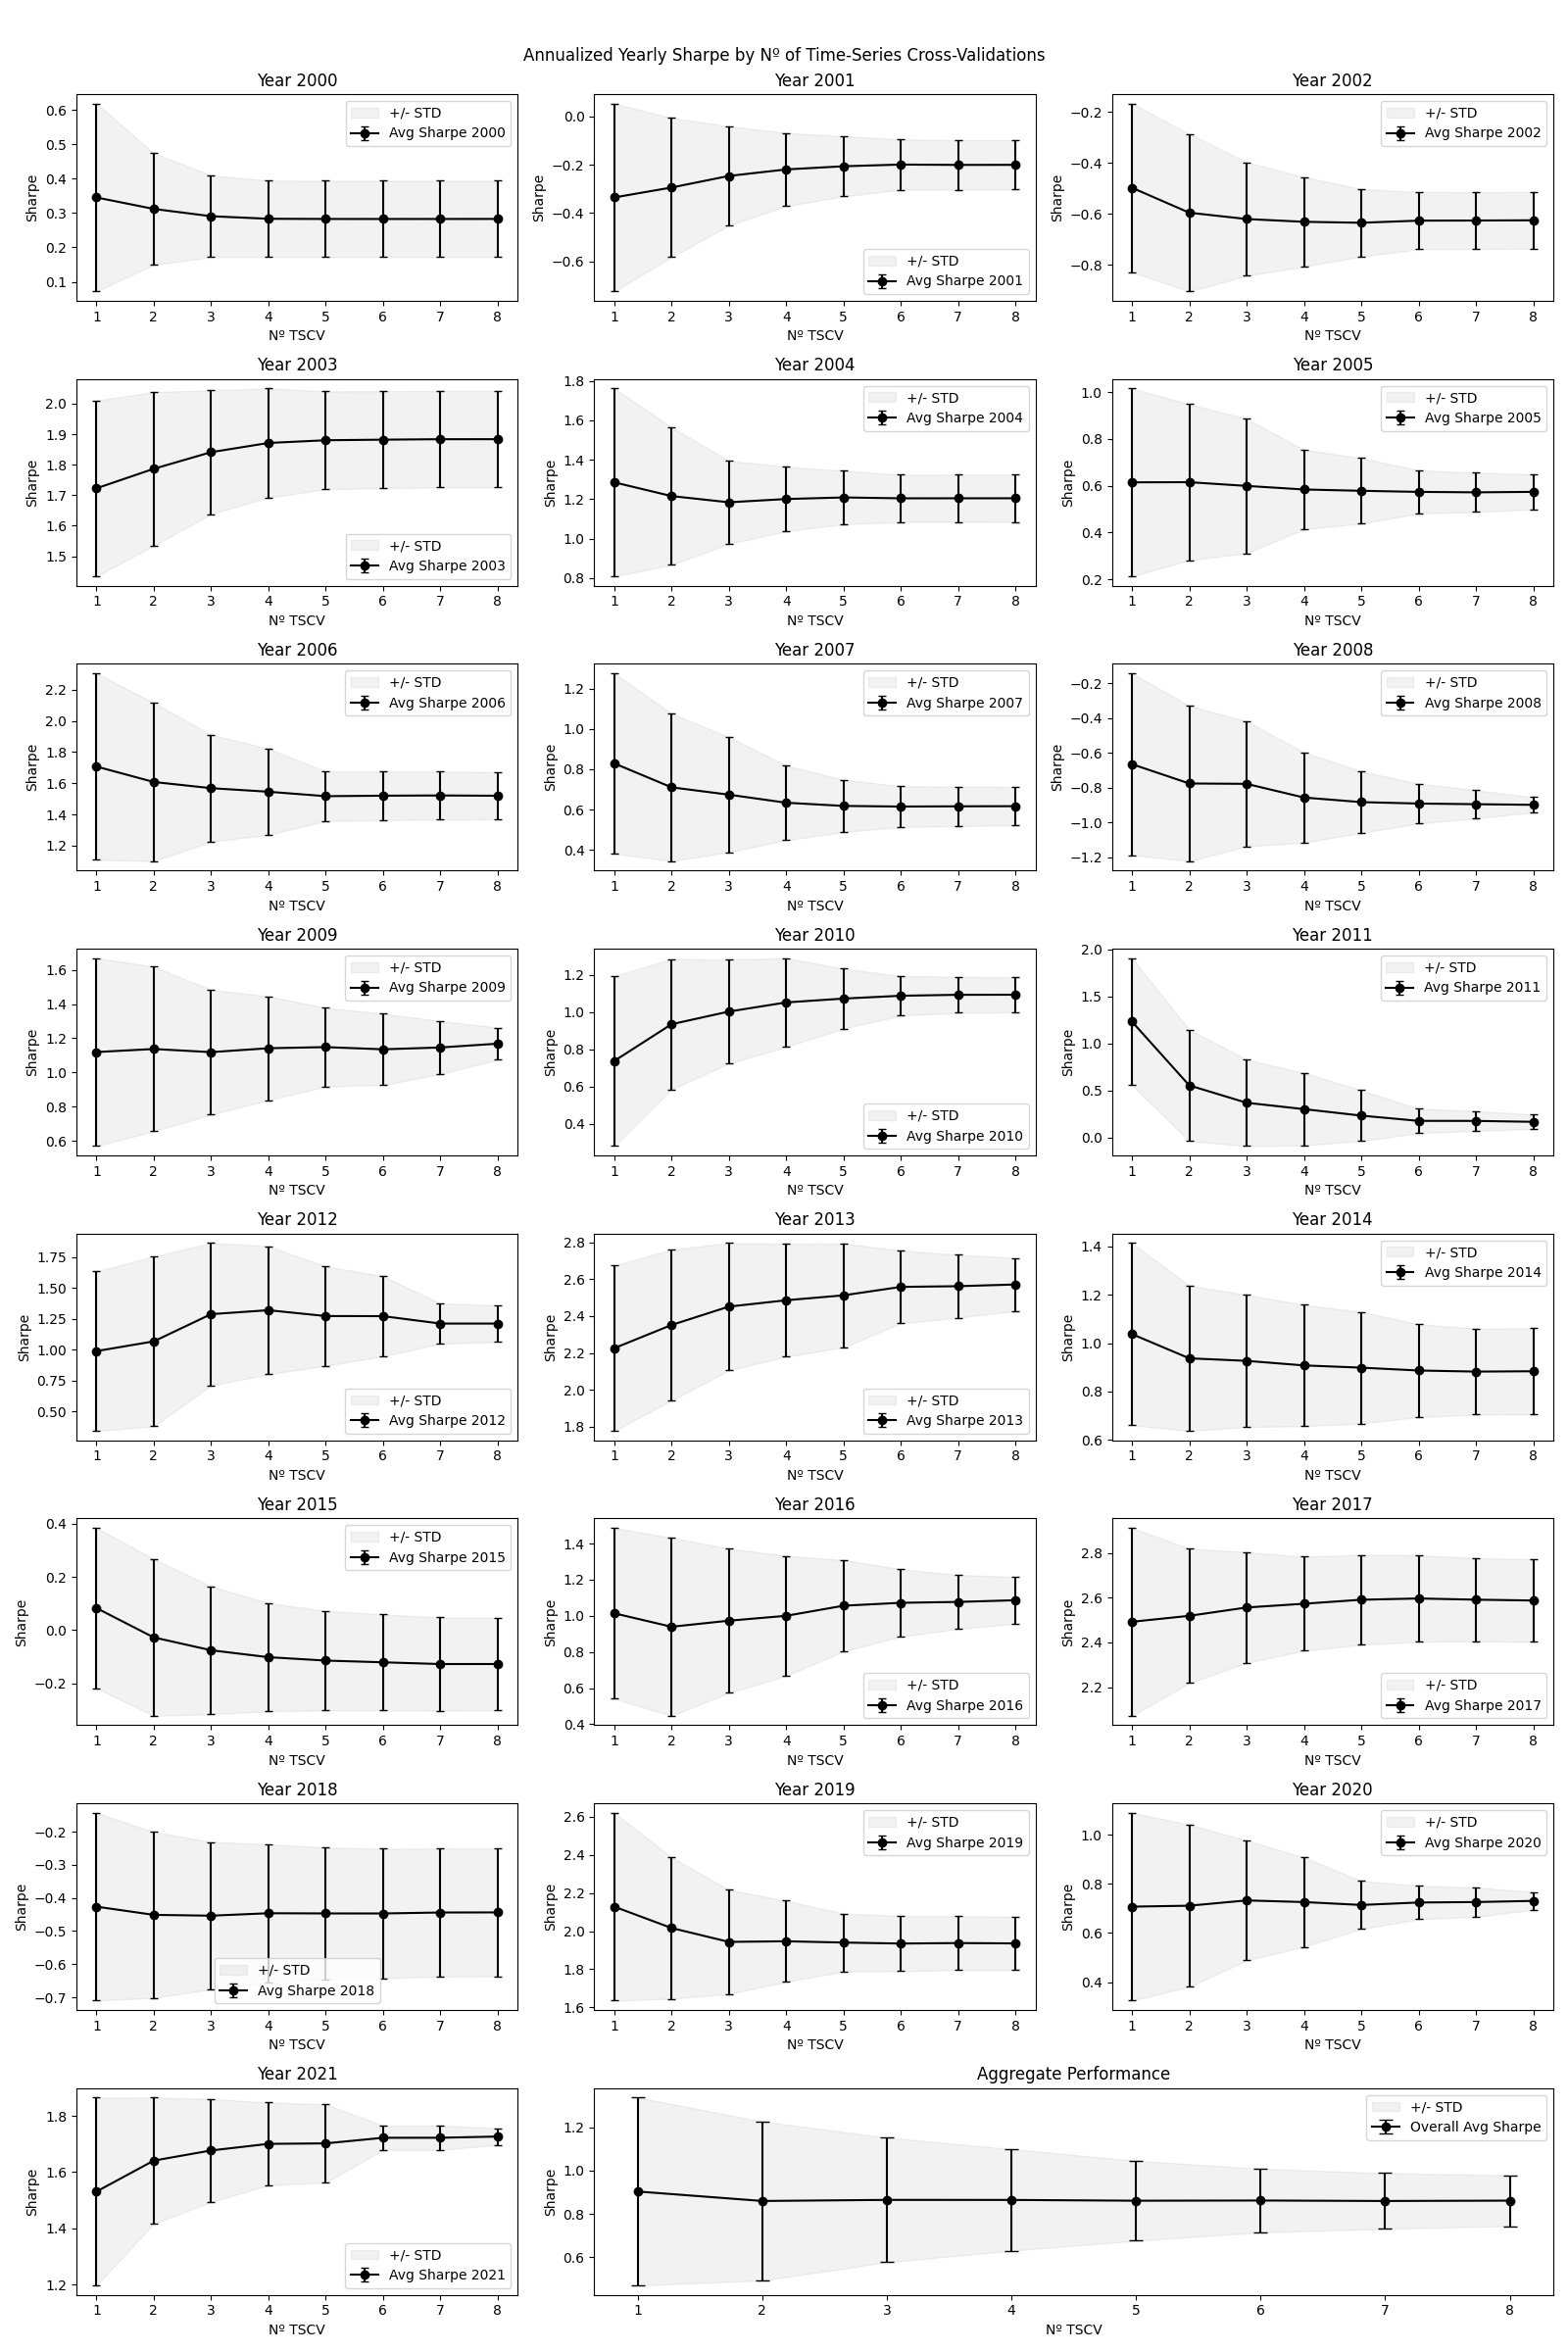
\includegraphics{graphics/time_series/n_tscv.png}
    }
    \caption{Sharpe by Nº of Time-Series Cross-Validations}
\end{figure}

\begin{figure}[h]
    \label{fig:time_series_testing_window}
    \centering
    \adjustbox{max size={\textwidth}{.90\textheight}}{
        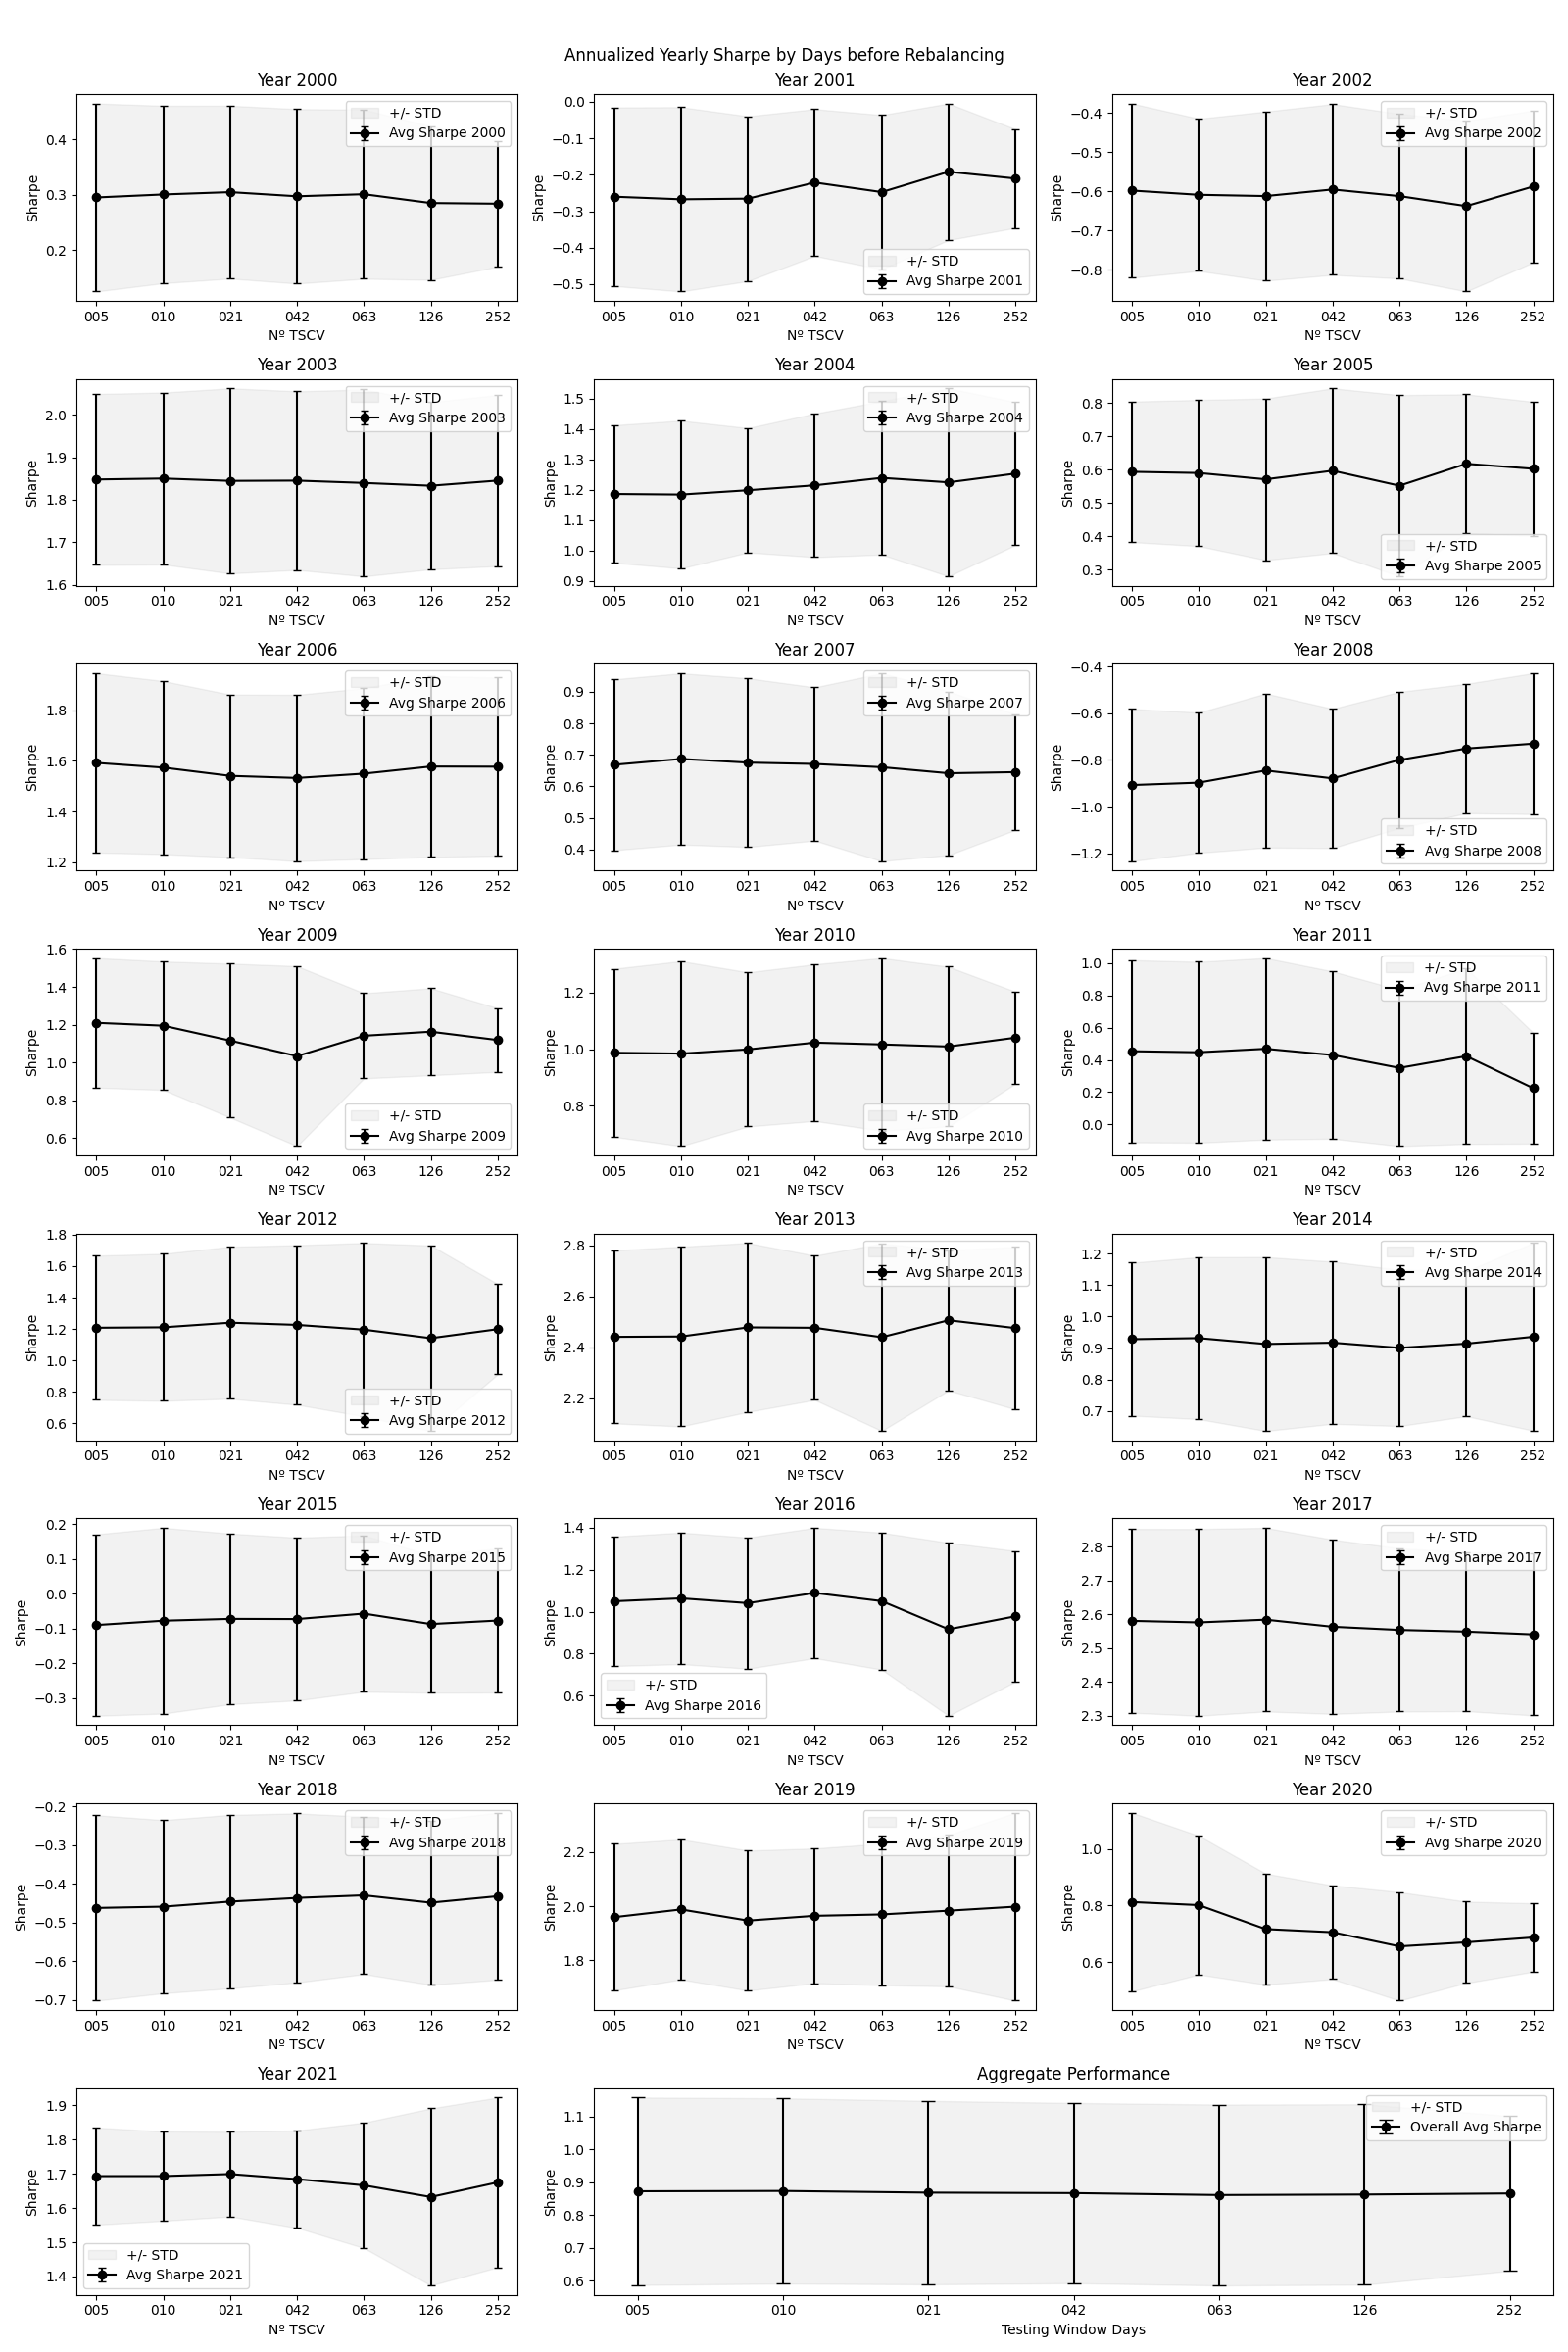
\includegraphics{graphics/time_series/testing_window.png}
    }
    \caption{Sharpe by Days before Rebalancing}
\end{figure}

\begin{figure}[h]
    \label{fig:time_series_training_window}
    \centering
    \adjustbox{max size={\textwidth}{.90\textheight}}{
        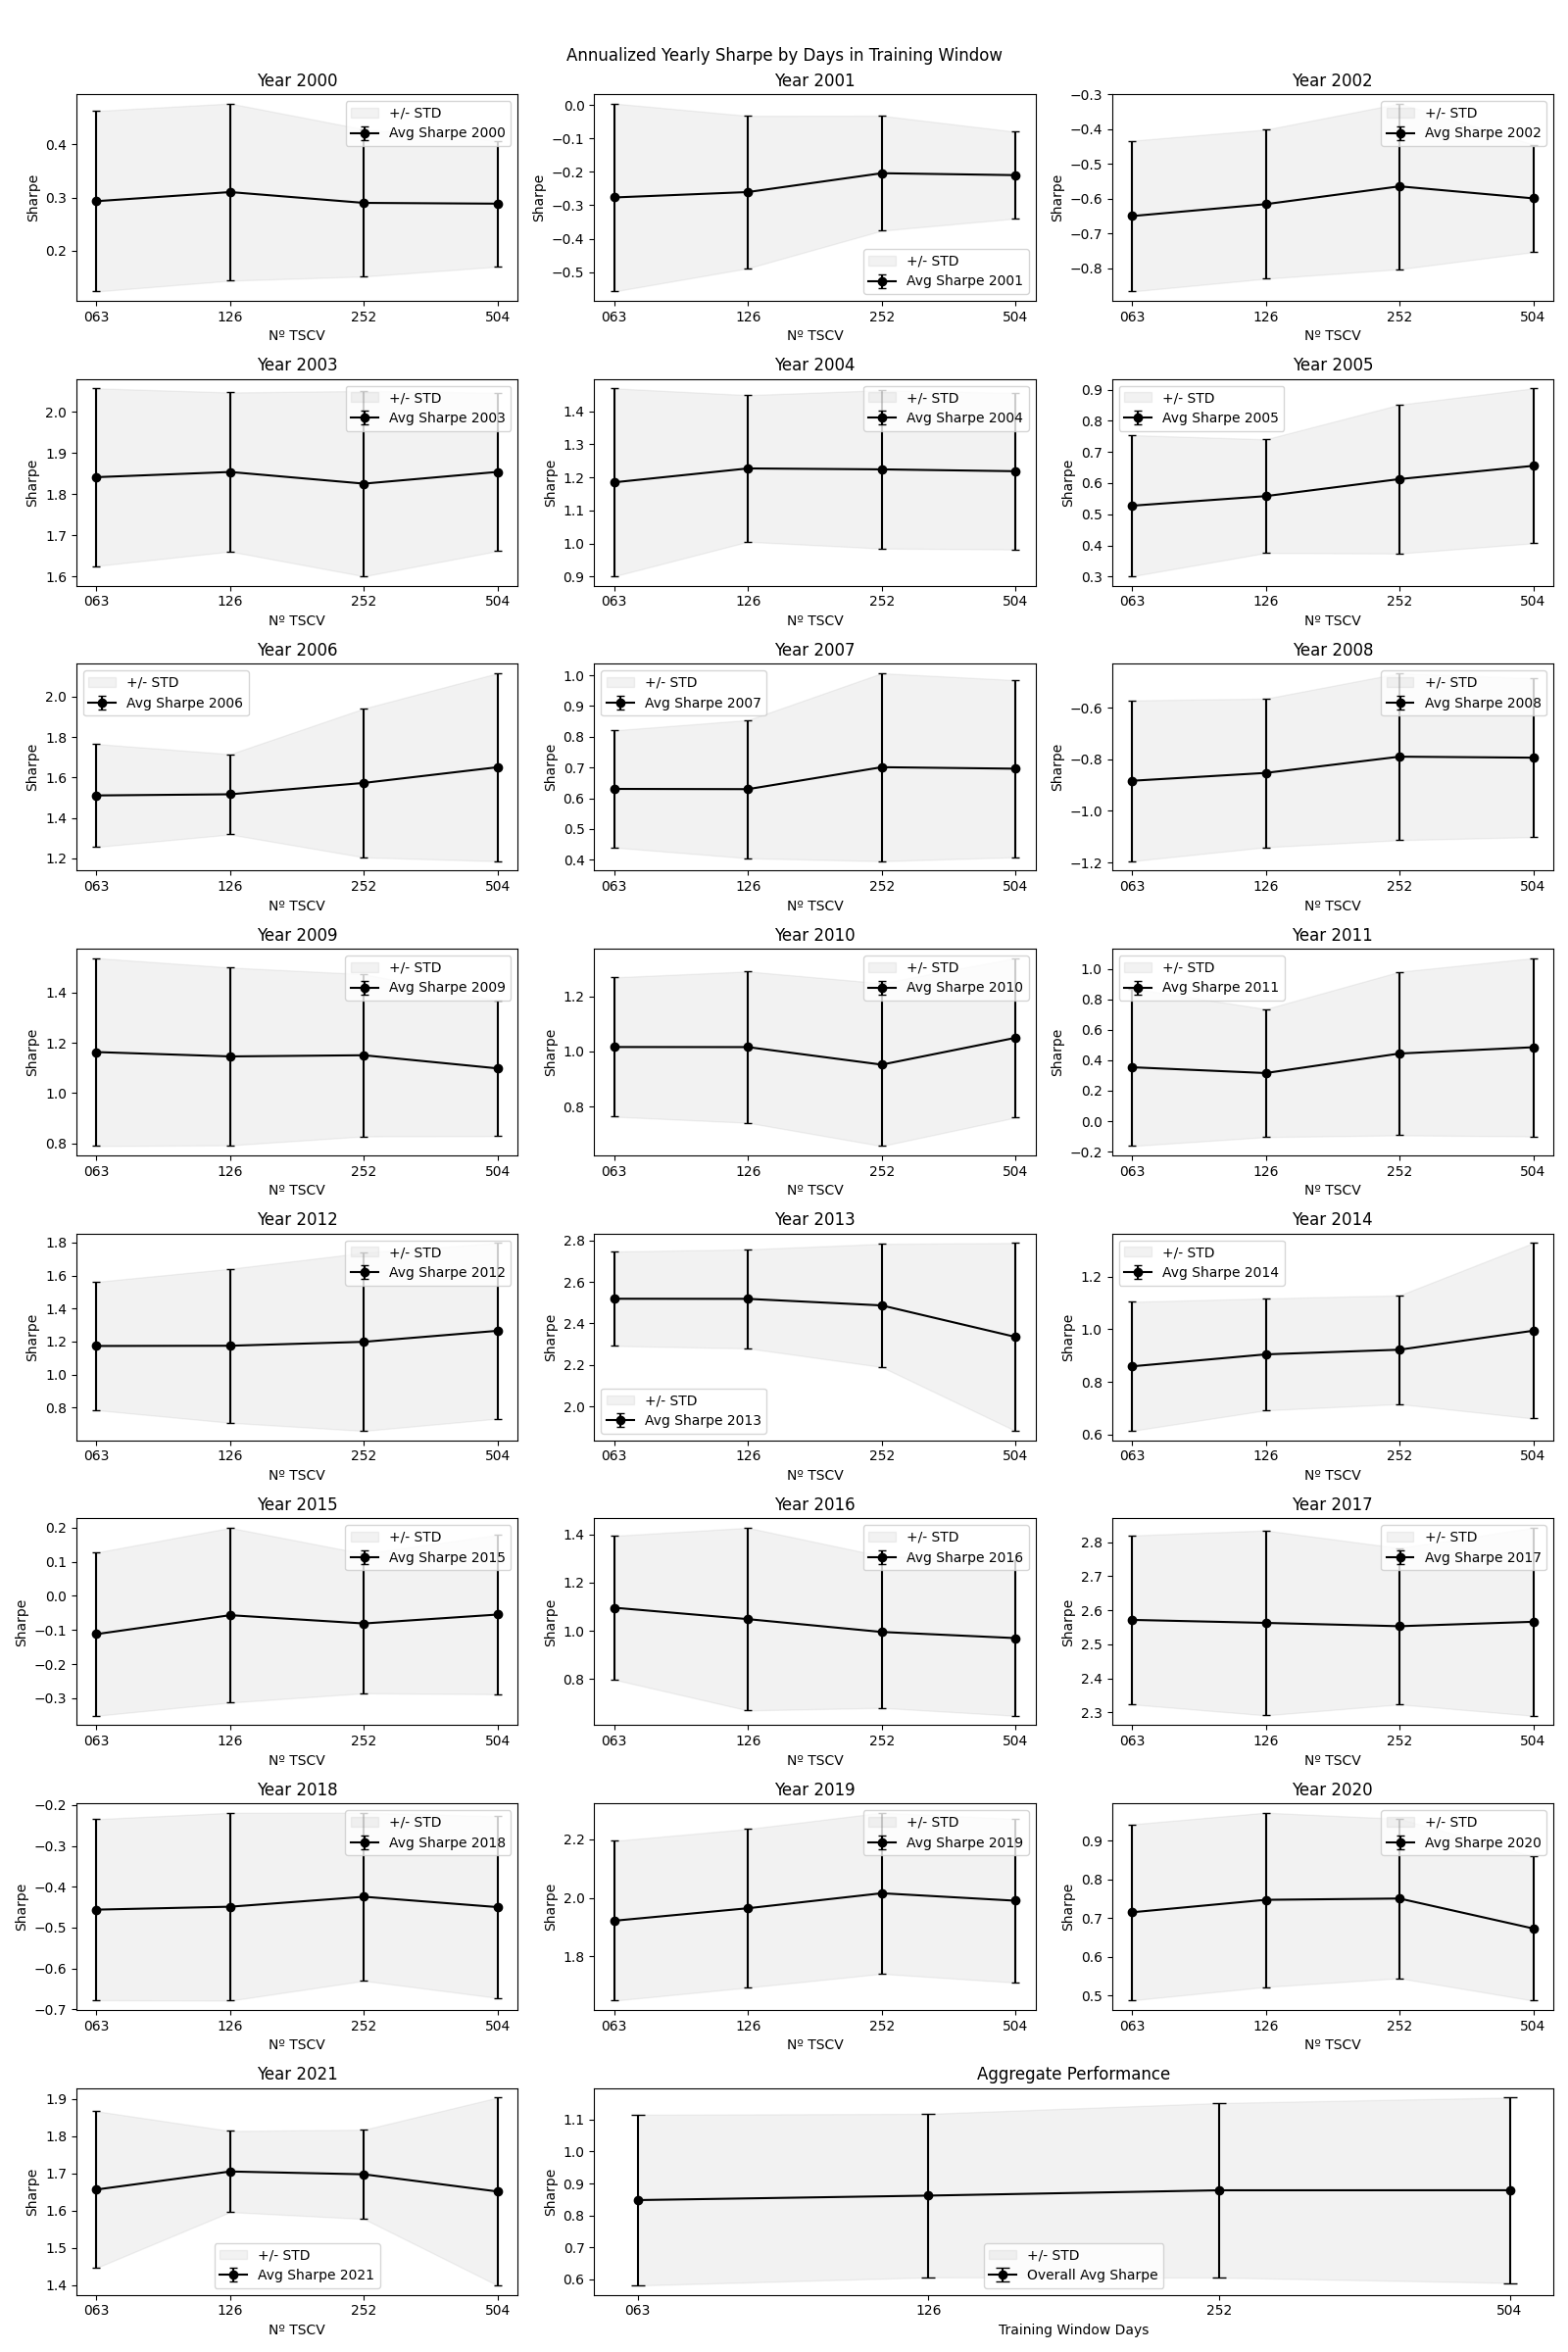
\includegraphics{graphics/time_series/training_window.png}
    }
    \caption{Sharpe by Days in Training Window}
\end{figure}

\begin{figure}[h]
    \label{fig:time_series_tscv_size_multiple}
    \centering
    \adjustbox{max size={\textwidth}{.90\textheight}}{
        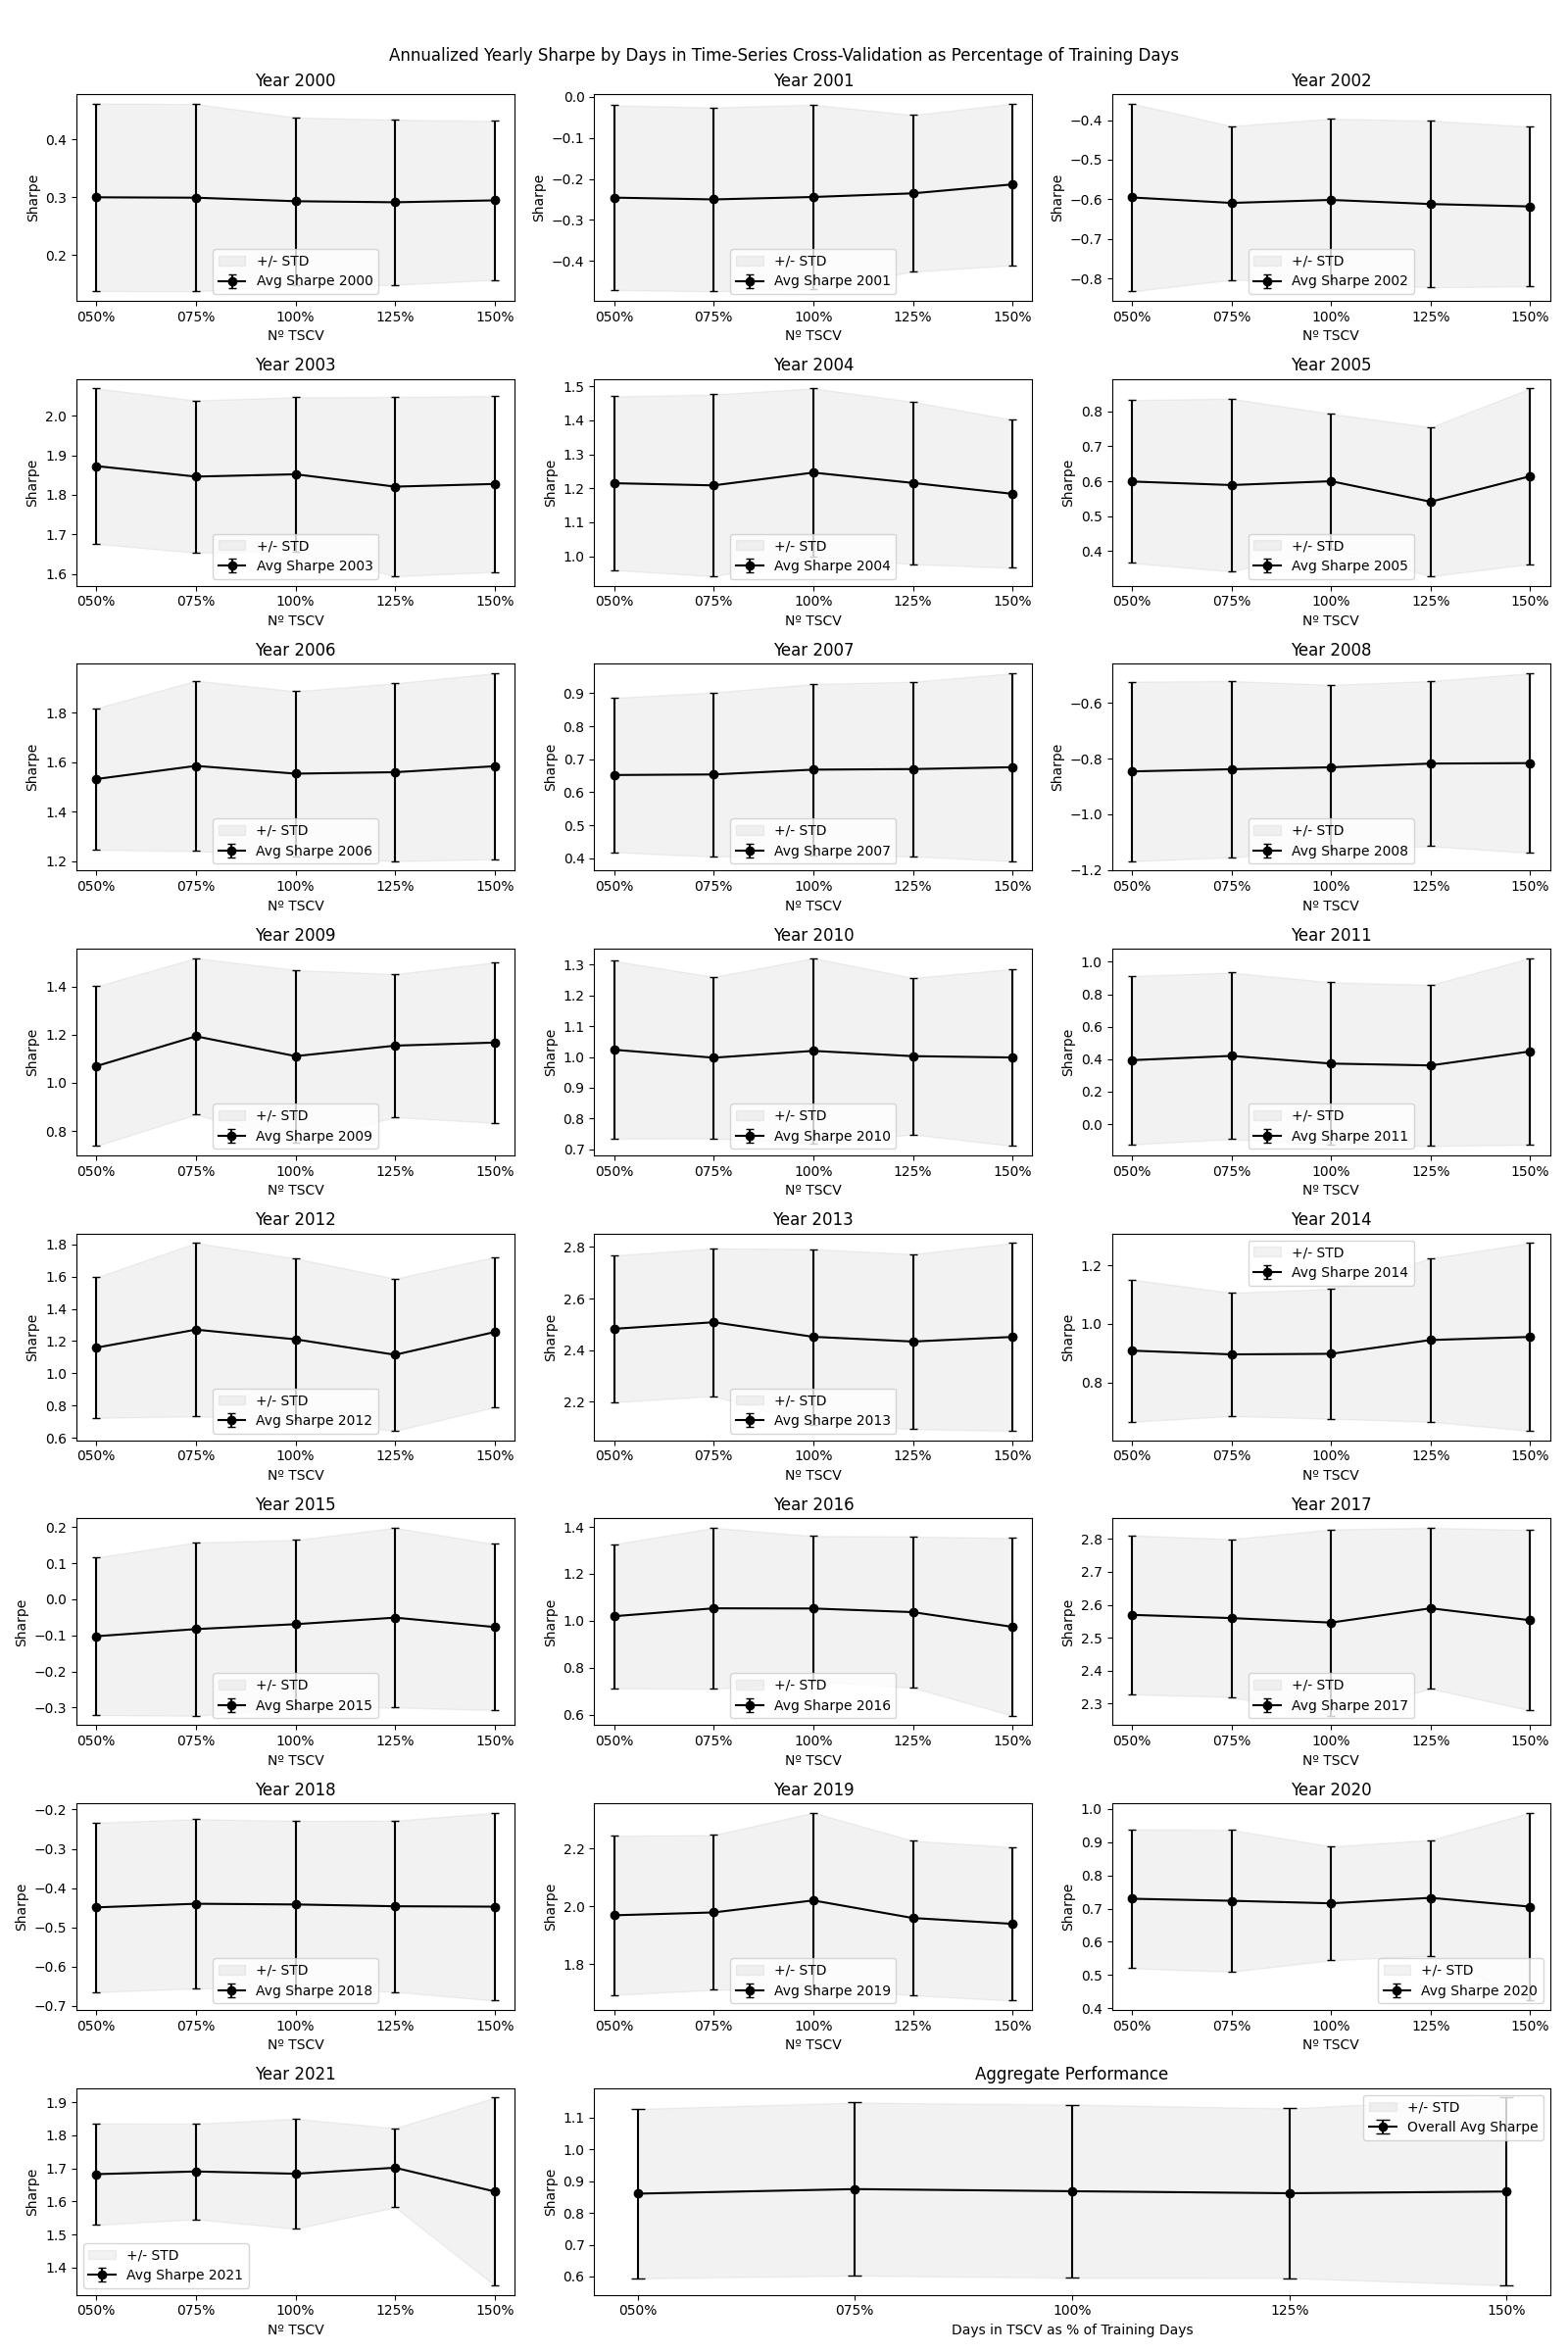
\includegraphics{graphics/time_series/tscv_size_multiple.png}
    }
    \caption{Sharpe by Days in Time-Series Cross-Validations as Percentage of Training Days}
\end{figure}

\begin{figure}[h]
    \label{fig:time_series_n_assets}
    \centering
    \adjustbox{max size={\textwidth}{.90\textheight}}{
        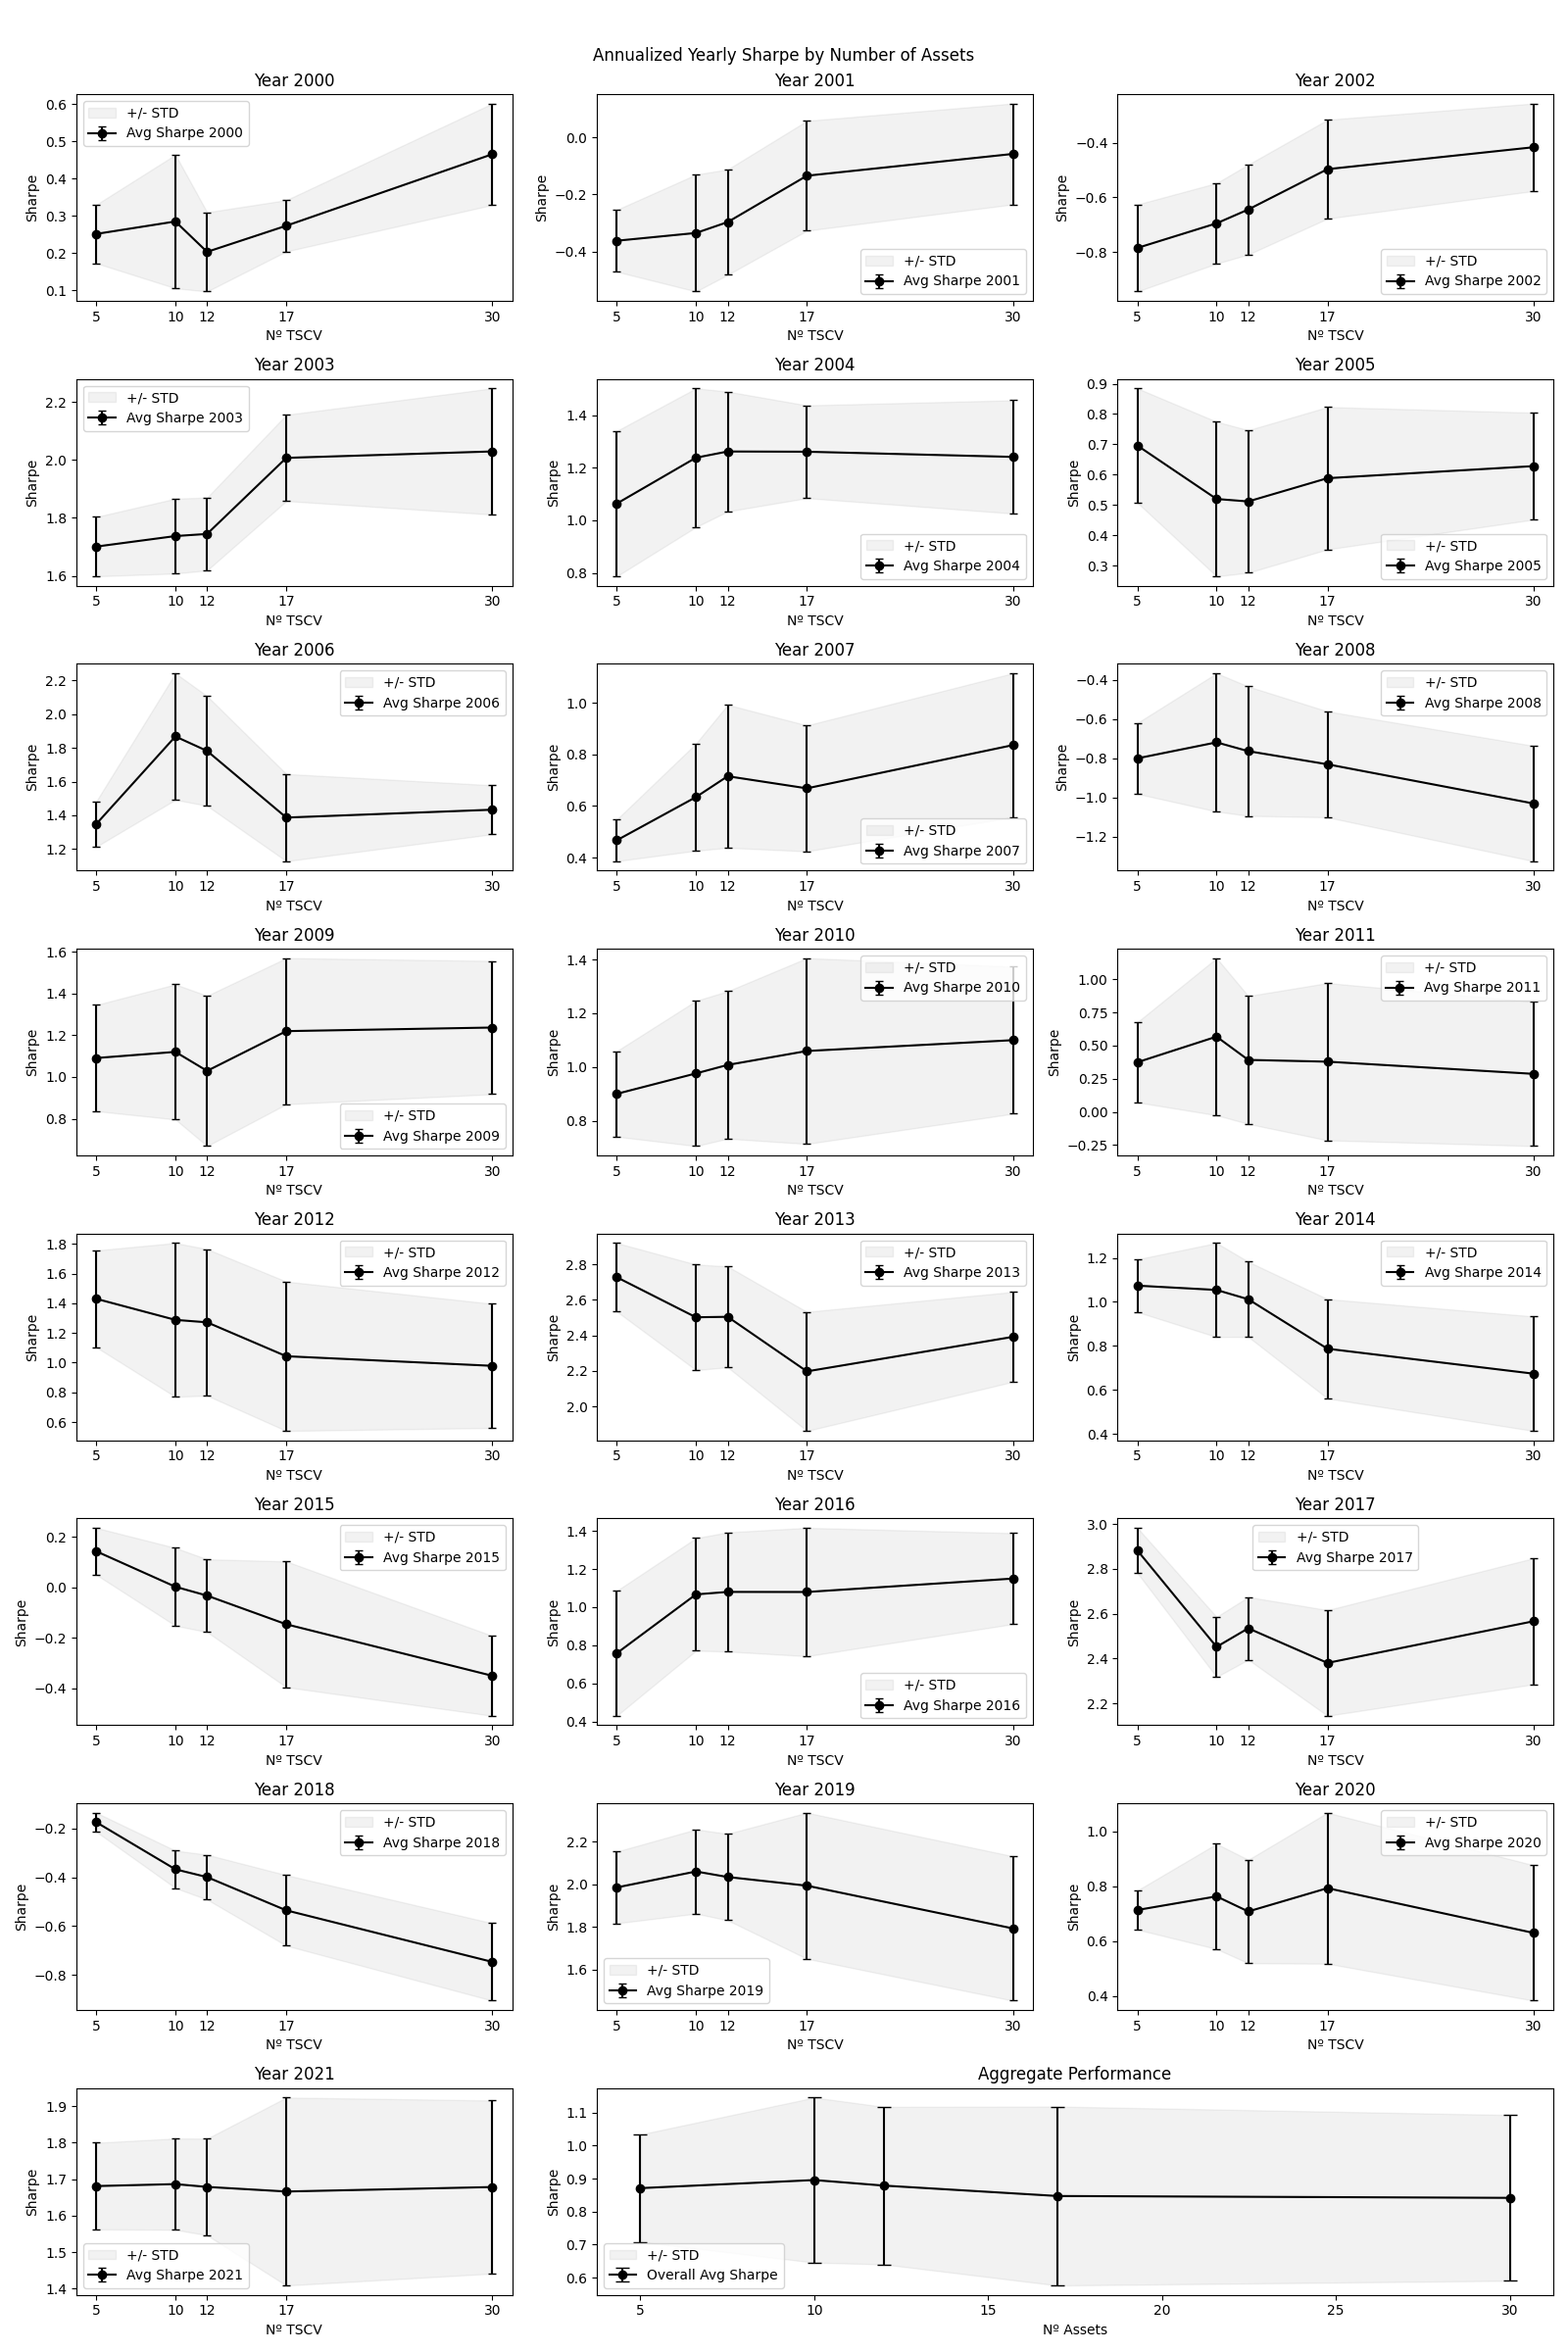
\includegraphics{graphics/time_series/n_assets.png}
    }
    \caption{Sharpe by Number of Assets}
\end{figure}

\end{document}